\myparagraph{Hypothèses}
\begin{itemize}
 \item L'échéancier a été conçu de façon à concilier ma vie de famille, mon travail, mes activités personnelles et la réalisation de mon essai.
 \item La revue de la littérature a déjà été commencée bien avant le début de la session.
 \item Le plan de travail a été complété pendant le cours GAE723 avant le début de la session.
 \item Les sources de données ont déjà été choisies et vérifiées.
 \item L'environnement de travail et de développement a déjà été choisi et évalué.
 \item Des prises de notes et brouillons sont prises au fur et à mesure de l'exécution, et mises à jour. Les parties qui peuvent être rédigées sans risque d'être retouchées peuvent être complétées. Sinon la rédaction finale et propre de l'essai sera faite dans la dernière partie de l'échéancier.
 \item L'inscription se fait à la session d'hiver.
 \item Le début de l'essai commence la deuxième semaine de janvier.
 \item L'inscription à l’essai est faite le 21 janvier.
 \item Le dépôt initial est planifié dans la semaine du 24 août.
 \item Le dépôt final est planifié dans la semaine du 28 septembre.
 \item L'essai se déroule sur deux sessions, hivers et été, échelonné sur une durée de 38 semaines.
 \item Il y a une semaine de pause d'incluse, pendant la semaine de relâche scolaires 29 mars. 
 \item Mes vacances d'été sont planifiées fin Août, du 14 août au 03 septembre.
 \item Le directeur a deux semaines pour réviser les parties qui lui sont remises. Un temps est alloué avec lui afin de réviser ses commentaires. 
 \item Il est planifié revoir l'échéancier régulièrement, surtout pour s'adapter aux événements non sollicités et inattendus.
\end{itemize}
\textit{une présentation de style Gant, liste des activités et des semaines; doit être lisible et tenir sur une page (landscape) lisible}
\begin{landscape}
   \begin{figure}
      \centering
      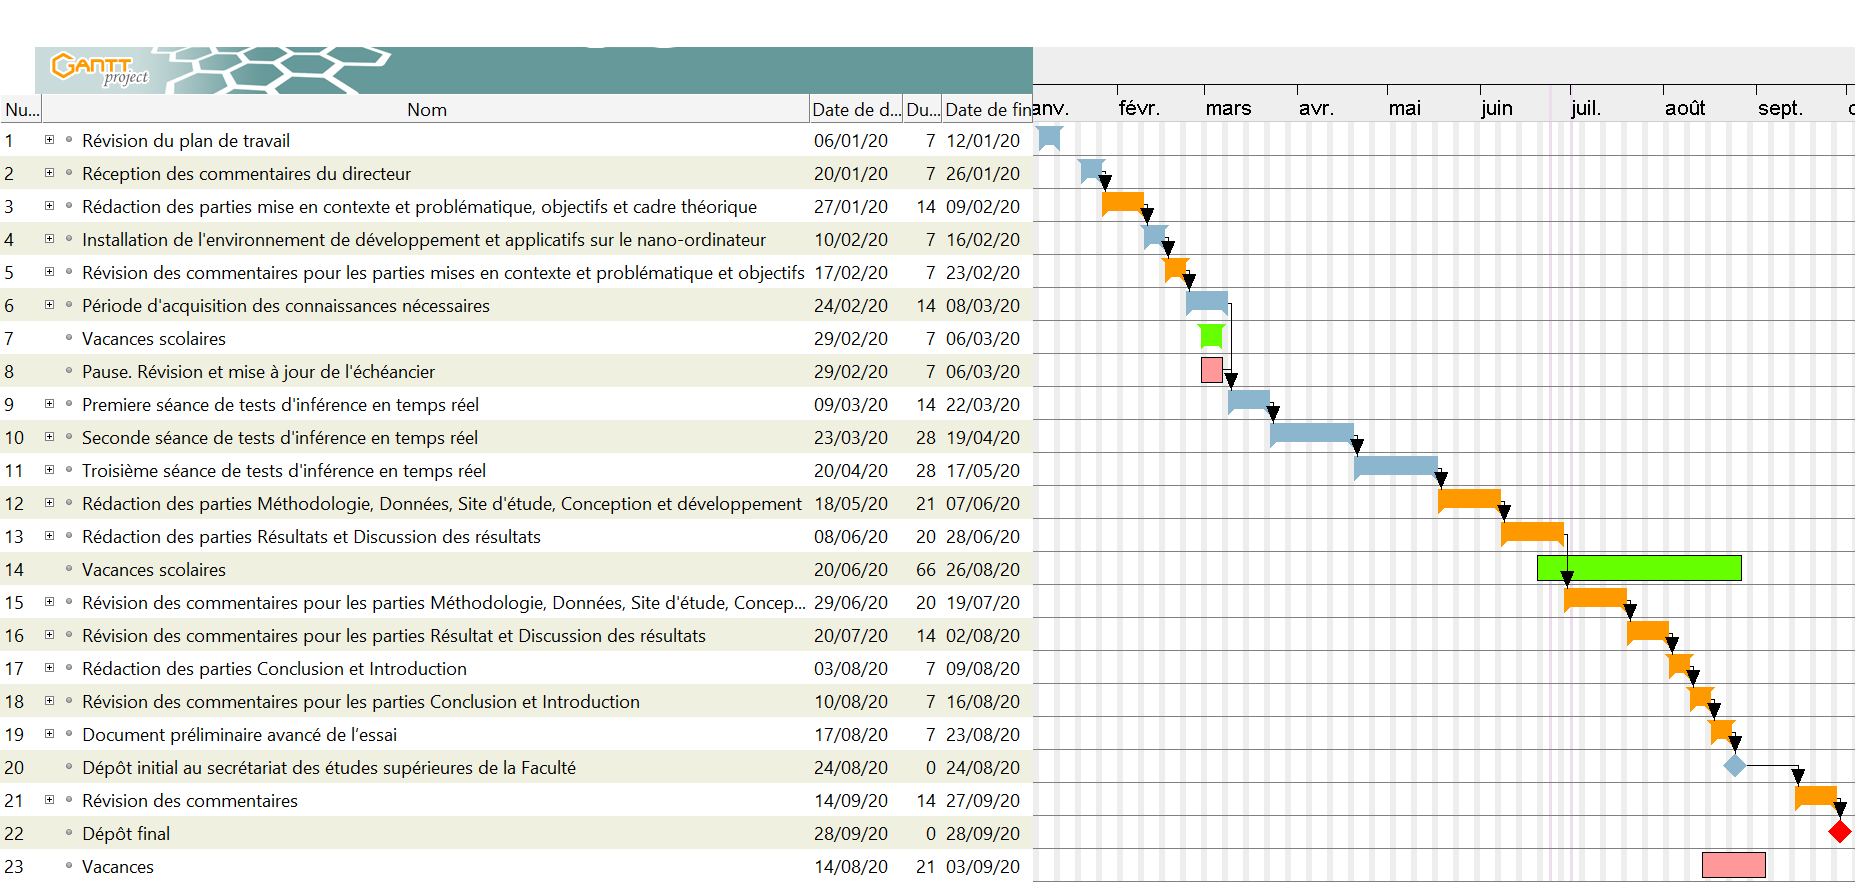
\includegraphics[width=1.4\textwidth, height=1.0\textheight]{echeancier}
      \caption{Échéancier}
      \label{fig:planning}
   \end{figure}
\end{landscape}
